\setcounter{section}{64}
\section{Персистентное дерево отрезков: определение, практическая значимость и реализация.}
\par \textbf{Определение:} \textit{Персистентные структуры данных} — это структуры данных, которые при внесении в них каких-то изменений сохраняют все свои предыдущие состояния и доступ к этим состояниям ("контроль версий").
\par Таким образом, персистентное дерево отрезков хранит все свои промежуточные состояния, то есть состояния после каждого запроса обновления. Однако, каждый раз оно не копируется: копируются только те вершины, в которых были произведены изменения, а остальные привязываются к ним указателями.
\begin{figure}[h]
    \centering
    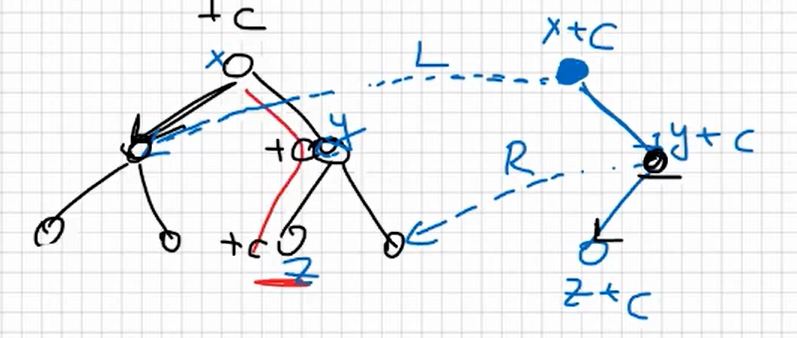
\includegraphics[scale=0.7]{images/65-66_persistent}
    \caption{Запрос обновления вершины $z$ в персистентном дереве отрезков}
\end{figure}
\par Реализовать это можно с помощью массива, в $i$-ой ячейке которого будет находиться указатель на корень $i$-ой версии дерева отрезков.
\par \textbf{Асимптотика:} обработка запроса изменения требует $O(\log n)$ времени и $O(\log n)$ дополнительной памяти, где $n$ - количество листьев. Таким образом, на всю программу нам потребуется $\Theta(n+q \log n)$ памяти, где $q$ - количество запросов.


\section{Количество чисел на отрезке, значения которых лежат в отрезке: решение с персистентным деревом отрезков.}
\par \textbf{Формулировка:} смотри билет 63
\par \textbf{Идея:} Считаем массив и отсортируем его (в отсортированном массиве будем хранить пары $(a_i, i)$). "Умертвим" все элементы и построим на исходном массиве дерево отрезков, в каждой вершине которого будет храниться количество "живых" элементов на отрезке. Затем будем идти по отсортированному массиву и "оживлять" элементы. Таким образом, $i$-ая версия дерева отрезков будет содержать все элементы $\leqslant a_i$, и мы легко сможем ответить на вопрос "сколько элементов лежит на отрезке $[l,r]$. Асимптотика построения: $O(n \log n)$
\begin{figure}[h]
    \centering
    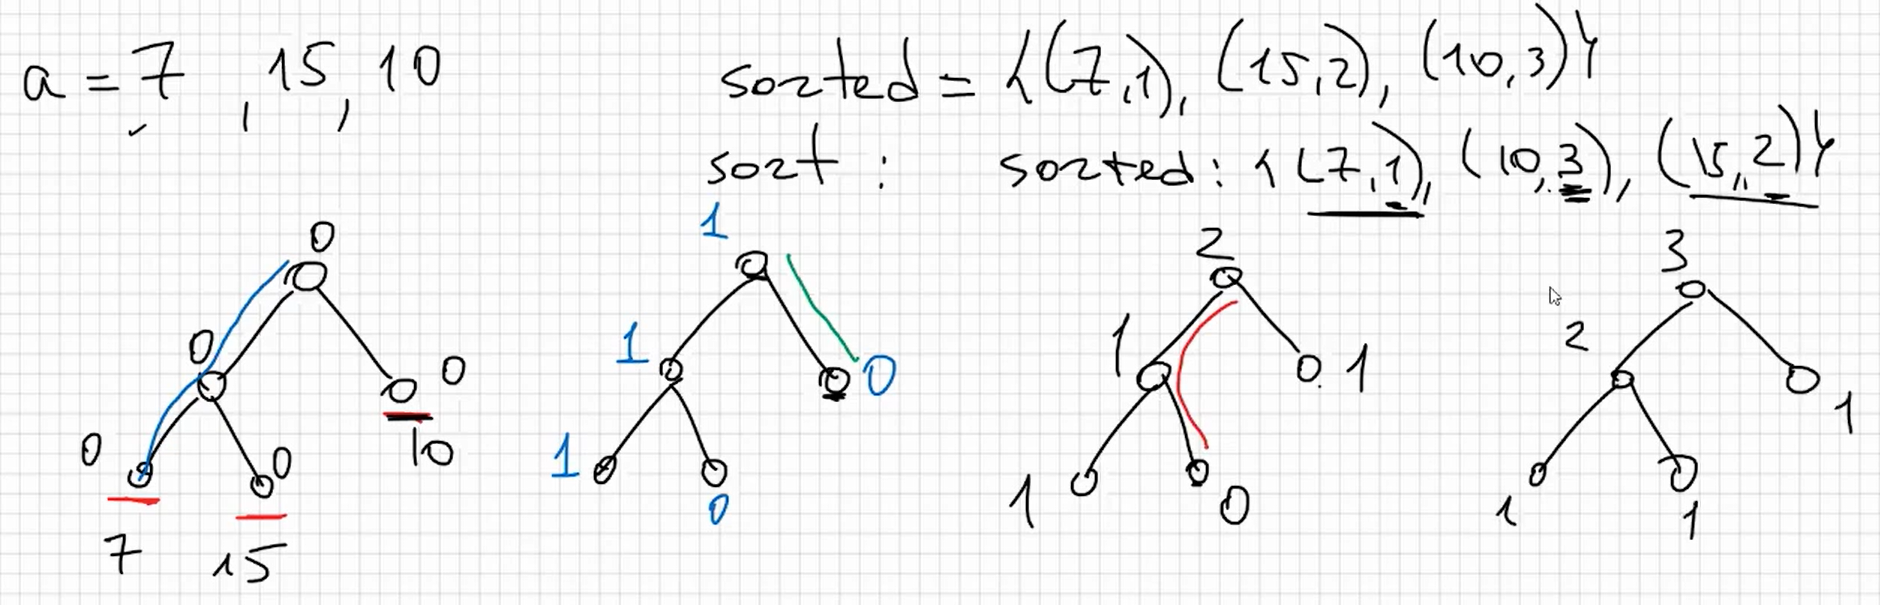
\includegraphics[width=\linewidth]{images/65-66_persistent task}
    \caption{Пример построения персистентного дерева для задачи}
\end{figure}
\par Тогда, когда нам приходит запрос мы \begin{enumerate}
    \item Бинарным поиском находим в отсортированном массиве позицию $i$ наибольшего числа $\leqslant y$. Асимптотика: $O(\log n)$
    \item Переходим в $i$-ую версию дерева отрезков и находим количество живых элементов на $[l,r]$. Это и будет наш ответ. Асимптотика: $O(\log n)$
\end{enumerate}
\par Таким образом, общая асимптотика - $O((n+q)\log n)$ времени и $O(n \log n)$ памяти, где $n$ - количество элементов, а $q$ - количество запросов